\documentclass{article}

\usepackage{setspace}
\usepackage{graphicx}
\usepackage[export]{adjustbox}
\usepackage{amsmath}
\usepackage{algorithm, algorithmic}%

\graphicspath{ {./imgs/} }

\title{Thesis Proposal: Escaping Local Minima using Symbols}
\author{Ahmed Galila\\ Jodrey School of Computer Science\\ Acadia University\\ Wolfville, NS, Canada, B4P 2R6\\ ahmedgalila@acadiau.ca}
\date{\today}

\begin{document}
	
	\maketitle
	
	\onehalfspace
	\setlength{\parskip}{\baselineskip}
	
	\begin{abstract}
		
		Many advances in artificial intelligence research have been attributed to our understanding of certain aspects of cognitive science. Deep learning is one such area inspired by how the human brain processes sensory input. The goal is to train predictive models using a hierarchal approach were each level is an abstraction of the layer below. This presents a challenge, since eventually the training process will reach a point where further modification will not provide noticeable improvements. Individual human learners encounter similar difficulties while learning. However, these challenges are overcome through social interaction and the sharing of learned knowledge. This thesis attempts to draw parallels between the human learning process and learning in neural networks. A hypothesis is presented where, similar to the effect of social interaction on the effectiveness of learning among humans, knowledge sharing in the form of symbolic data between artificial neural networks can also improve effectiveness (accuracy) of learning within these networks. Several empirical studies with a focus on learning with symbols using noisy handwritten digits will be presented and an analysis of the results will be provided. 
		
	\end{abstract}
	
	\section{Introduction}
	
	\subsection{Synopsis} \label{sec:introduction-synopsis}
	
	Many advances in artificial intelligence (AI) research are inspired by work done in other fields, specifically those that aim to study human cognition, language and social interaction\cite{DBLP:journals/corr/abs-1203-2990}. Deep learning is one particular area of AI that is heavily influenced by how the human brain works. It borrows from the fact that our nervous system processes sensory input via a multi layer hierarchy of neurons\cite{DBLP:journals/corr/abs-1203-2990}. In deep learning, artificial neural network models are constructed using multiple layers of artificial neurons and used to represent complex phenomena that are difficult to capture using tradition algorithms\cite{Bengio:2009:LDA:1658423.1658424}. For example a neural network can be constructed and trained to identify objects in a digital image, a task that would be too complex to accomplish using traditional programming languages.
	
	In order to capture the complexity of such tasks, predictive models (models that predict output from previously unobserved data points) must be constructed several layers deep. Training deep architectures however, presents its own unique challenges. One such challenge is the difficulty of the training algorithm to find a suitable global minimum in the solution space due to the presence of many local minima\cite{Larochelle:2009:EST:1577069.1577070}.
	
	When considering how learning in humans work, it is believed that the ability of individual humans to learn new concepts accurately, is hampered by the number and variety of examples of the concepts they are each exposed to\cite{DBLP:journals/corr/abs-1203-2990}. This can be associated with how the existence of many local minima in the solution space of a deep neural network prevents it from converging on the desired solution. However, this difficulty is overcome when individuals communicate examples of concepts and knowledge between each other in a social structure\cite{DBLP:journals/corr/abs-1203-2990}. In a society, a common method of communication is developed, that significantly improves the efficiency and effectiveness of the learning process.
	
	Drawing from that analogy, we can hypothesise that similar to how human learners use knowledge that is transfered using a common language to overcome difficulty in learning from limited examples, artificial neural networks can also benefit from a clear knowledge representation to improve the effectiveness (accuracy) of training using a limited dataset.
	
	\subsection{Research Objective}
	
	Our goal is to draw parallels between our understanding of how humans learn and how various machine learning techniques work. The objective is to demonstrate that having a clear representation of knowledge within deep neural networks can improve the effectiveness of the training process by significantly reducing the number of training examples needed to produce a high level of accuracy.
	
	This knowledge sharing will be demonstrated in my thesis by training deep neural networks to perform basic arithmetic operations (such as addition) on images of handwritten digits. These models will accept the images as inputs and will output the result of the operation. The models will also accept a symbolic input channel, depicted as a clean image of the same input digits rendered using a standard font, representing the shared knowledge. Training will be performed with and without the presence of the symbolic input. The results will then be analyzed to show the impact of the symbolic channel on the accuracy of the models developed.
	
	Our understanding is that in deep neural networks, arbitrary areas of the architecture learn abstractions that can be shared among different tasks\cite{Bengio:2009:LDA:1658423.1658424}. There are some commonalities in learning using noisy images and symbols. Parts of the models should be able to successfully represent these commonalities, and since it is easier to learn using symbols, the symbolic channel when present during training would make it easier for the network to achieve these abstractions and therefore increase the accuracy of the model when applied to noisy (handwritten) inputs alone.
	
	\subsection{Scope}
	
	My research will investigate the effect of using clear symbolic information on the effectiveness of artificial neural networks. A background in machine learning as it relates to neural networks will be provided. The problem of local minima will also be discussed. In the process several neural network models will be developed, tested and analyzed. The thesis will not go into details of any of the natural sciences related to the topic such as neurology or sociology.
	
	\section{Background}
	
	\subsection{Deep Learning}
	
	Designing computer systems that can model the world in such a way as to exhibit what we call intelligence, for example identifying objects in images, requires such systems to have the ability to interpret a large number of factors. Given the amount of data required, it would be infeasible to manually formalize solutions to these problems. Learning algorithms can instead be used to learn the important factors that represent the problem domains and formalize them in a way that can then be applied to different instances of the problem\cite{Bengio:2009:LDA:1658423.1658424}.
	
	Deep learning is an area of research where algorithms are developed that can learn these representations by building layers of processing units where each layer represents a certain level of abstraction, each layer more abstract than the layer below it\cite{Bengio:2009:LDA:1658423.1658424}. For example a model that can be used to identify objects in an image can be constructed in several layers. One layer learns to identify edges, the next layer learns to identify shapes all the way up to the final layer (output layer) that makes the actual classification.
	
	The processing units that make up these deep architectures are called artificial neurons, since they are inspired by how the neural networks in living organisms operate. The following section provides a brief overview of how these artificial neural networks learn to represent solutions to complex problems.
	
	\subsection{Artificial Neural Networks}
	
	\subsubsection{Artificial Neurons and Gradient Descent Algorithm}
	
	Consider the problem of classifying a set of data points into one of several classes. We can reduce this problem to that of finding a function $f(x)$ that approximates $y$, where $x$ is a vector representing the data points and $y$ is the class. That function $f(x)$ can be represented as a linear combination of the parameters of $x$:
	\begin{gather*}
	w_1 x_1 + w_2 x_2 + ... + w_n x_n + b = y_1\\
	w_1 x_1 + w_2 x_2 + ... + w_n x_n + b = y_2\\
	\vdots\\ 
	w_1 x_1 + w_2 x_2 + ... + w_n x_n + b = y_m
	\end{gather*}
	The problem of learning the decision function becomes finding a set of weights ($w_1$ to $w_n$ and $b$) that satisfy the provided data points as well as generalize to yet unseen observations\cite{Le15atutorial}. This system of equations can be depicted as a neuron, like that shown in figure \ref{fig:perceptron}, that accepts inputs and fires an output that is modified by weights, representing the synaptic weights in neural networks found in living organisms. Once fully trained, the neuron (also called a perceptron) is then used to predict the output of unseen observations using the following formula:
	\begin{gather}
		z = b + \sum\limits_{i=1}^n x_i w_i\\
		y = \frac{1}{1+e^-z}
	\end{gather}
	
	\begin{figure}
		\centering
		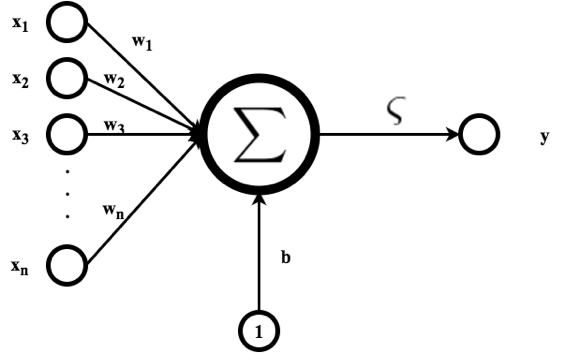
\includegraphics[max width=\textwidth]{perceptron}
		\caption{Visual depiction of a single artificial neuron, sometimes called a perceptron.}
		\label{fig:perceptron}
	\end{figure}
	
	The process of discovering the optimum set of weights is performed using the gradient descent algorithm. Gradient descent involves updating the weights of the model in such a way as to minimize the error produced by  applying the training examples to the perceptron relative to the expected target output. The error is depicted as a cost function whose gradient we need to traverse in the negative direction to minimize the error (figure \ref{fig:gradient-descent})\cite{Le15atutorial}. The mean square error (MSE) is a popular cost function\cite{Mitchell} given by:
	\begin{equation}
		E(\vec{w}) = \frac{1}{2} \sum_{d \in D} (t_d - y_d)^2
	\end{equation}
	where $\vec{w}$ are the neuron's weights, $D$ is the set of training examples, $t_d$ is the target output for the training example and $y_d$ is the actual output of the perceptron. 
	
	Figure \ref{fig:gradient-descent} visualizes the error function. Initially the weights are set to random values that place the error at an undesirable level. By iteratively updating the weights the error is reduced and the weights evolve to capture the decision function. The weight update rule is given by:
	\begin{equation}
		w_i \leftarrow w_i + \Delta w_i
	\end{equation}
	where
	\begin{equation}
		\Delta w_i = -\eta \frac{\partial E}{\partial w_i}
	\end{equation}
	$\eta$ is the learning rate. The learning rate is a positive value that determines the step size that the gradient descent will take. The larger the learning rate the quicker the descent, however this risks skipping the optimum weights.
	
	The change $\Delta w_i$ can be obtained by partially differentiating the error with respect to $wi$:
	\begin{equation}
		\begin{split}
			\frac{\partial E}{\partial w_i} & = \frac{\partial}{\partial w_i} \frac{1}{2} \sum_{d \in D} (t_d - y_d)^2\\
			& = \frac{1}{2} \sum_{d \in D} \frac{\partial}{\partial w_i} (t_d - y_d)^2\\
			& = \frac{1}{2} \sum_{d \in D} 2(t_d - y_d) \frac{\partial}{\partial w_i} (t_d - y_d) \\
			& = \sum_{d \in D} (t_d - y_d) \frac{\partial}{\partial w_i} (t_d - \vec{w}.\vec{x_d}) \\
			& = \sum_{d \in D} (t_d - y_d) (-x_{id})
		\end{split}
	\end{equation}
	where $x_{id}$ is the input of training example $d$. The update rule is therefore given by:
	\begin{equation}
		\Delta w_i = \eta \sum_{d \in D} (t_d - y_d) (x_{id})
	\end{equation}
		
	\begin{figure}
		\centering
		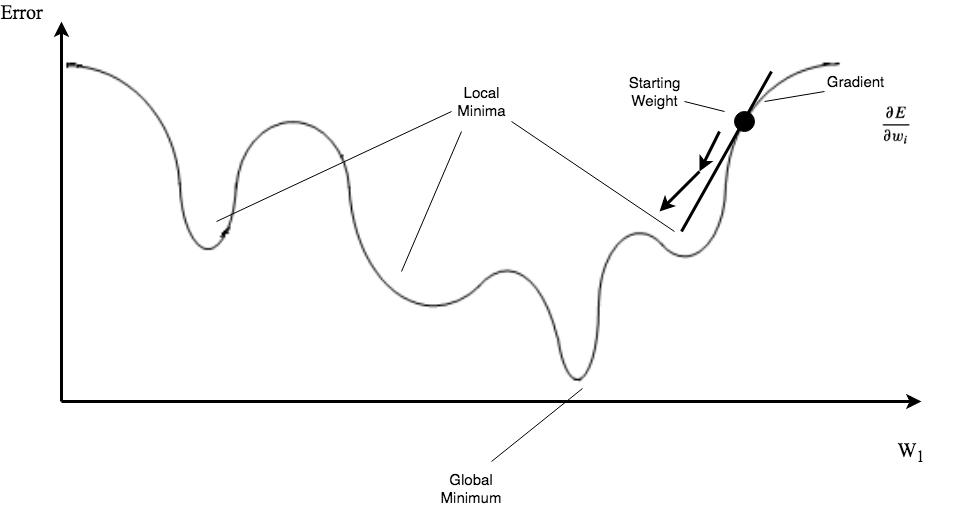
\includegraphics[max width=\textwidth]{gradient-descent}
		\caption{Weights are updated to minimize the error produced by the cost function in an effort to reach the global minimum.}
		\label{fig:gradient-descent}
	\end{figure}
	
	\subsubsection{Feed Forward Network and Backpropagation Algorithm}
	
	A single neuron is limited to only discovering linear decision functions as show in figure \ref{fig:separation-surface}(a). However, many real world problems are too complex to be modeled using a linear function as seen in figure \ref{fig:separation-surface}(b). Instead, individual neurons can be combined together into several layers to form a topology known as a feed forward network like the one in figure \ref{fig:feed-forward}. Feed forward networks are composed from one ore more fully connected layers, an output layer and zero or more hidden layers\cite{Mitchell}. By increasing the complexity of the network, the number of weights increases and therefore the separation surface produced by the model also increases in complexity\cite{Bengio07scalinglearning}.
	
	\begin{figure}
		\centering
		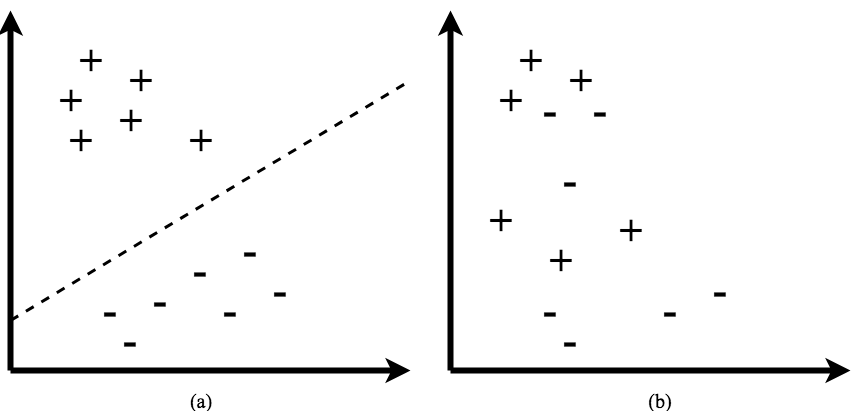
\includegraphics[max width=\textwidth]{separation-surface}
		\caption{A linear decision function (a) can not represent models that can solve more complex problems (b).}
		\label{fig:separation-surface}
	\end{figure}
	
	Feed forward networks are trained similar to how a single neuron is, by running the training dataset through the network and minimizing the error between the outputs and the expected results. Gradient descent is also used to find the approximate weights that will minimize the value of the cost function. However, applying gradient descent to feed forward networks is slightly more involved given the complex nature of the model.\cite{Le15atutorial}.
	
	\begin{figure}
		\centering
		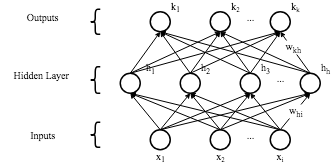
\includegraphics[max width=\textwidth]{feed-forward}
		\caption{A feed forward neural network with a single hidden layer.}
		\label{fig:feed-forward}
	\end{figure}
	
	The Backpropagation Algorithm is used to apply gradient decent to the individual units of the network\cite{Mitchell}. Initially the network weights are set to random values. Then for each training example, the backpropagation algorithm goes through two stages. First the input is propagated forward and the output $o_u$ of every unit $u$ is calculated. Next comes the backpropagation part where errors are propagated backwards through each layer and new weights are calculated.
	
	For each output unit $k$ an error term $\epsilon_k$ is calculated
	\begin{equation}
		\epsilon_k \leftarrow o_k (1 - o_k)(t_k - o_k)
	\end{equation}
	where $o_k$ is the actual output of the output unit $k$ and $t_k$ is the target for output unit $k$. Then the error $\epsilon_h$ for each hidden unit $h$ is calculated
	\begin{equation}
		\epsilon_k \leftarrow o_h (1 - o_h) \sum_{k \in outputs} w_{kh} \epsilon_k
	\end{equation}
	where $o_h$ is the output from hidden unit $h$ and $w_{kh}$ is the weight of the connection between the hidden unit $h$ and the output unit $k$. Finally the weight of the connection from unit $i$ to unit $j$ is updated using the following update rule
	\begin{equation}
		w_{ji} \leftarrow w_{ji} + \eta \epsilon_j x_{ji}
	\end{equation}
	
	\subsection{The Problem of Local Minima}
	
	Combining more units together to form a neural network may increase the expressiveness and accuracy of the model. However, this adds more challenges to the training process. Figure \ref{fig:gradient-descent} depicts the loss function against the value of the weights. The complex topology of the feed forward network adds regions in the loss function that act as local minima. This makes it more likely for the backpropagation algorithm to converge the weights to one of these local minima instead of the desired global minimum\cite{Larochelle:2009:EST:1577069.1577070}.
	
	Overcoming this difficulty in training can be achieved by increasing the number of training examples used. Other techniques involve pre-training the network using unsupervised learning first before using the network as a classifier as described in the next section\cite{Larochelle:2009:EST:1577069.1577070}. In this thesis however, we investigate how this problem can be overcome by introducing a symbolic channel to the network which is similar to how humans share knowledge.
	
	\subsection{Sequence Modeling}
	
	So far, we investigated machine learning models that assume independence between the individual training or test examples. After every data point is processed, the network resets its state and ignores any relationship between the new data point and previous data points. This works well for certain types of problems. However, not all problems exhibit this independence between the data points. For example, an autonomous vehicle that learns to move by analyzing sequences of frames from a video, might depend on previous frames in the input sequence to infer context. It is therefore important to extend the traditional neural network models to consider temporal information alongside spatial information\cite{DBLP:journals/corr/Lipton15}.
	
	\subsubsection{Recurrent Neural Networks}
	
	\begin{figure}
		\centering
		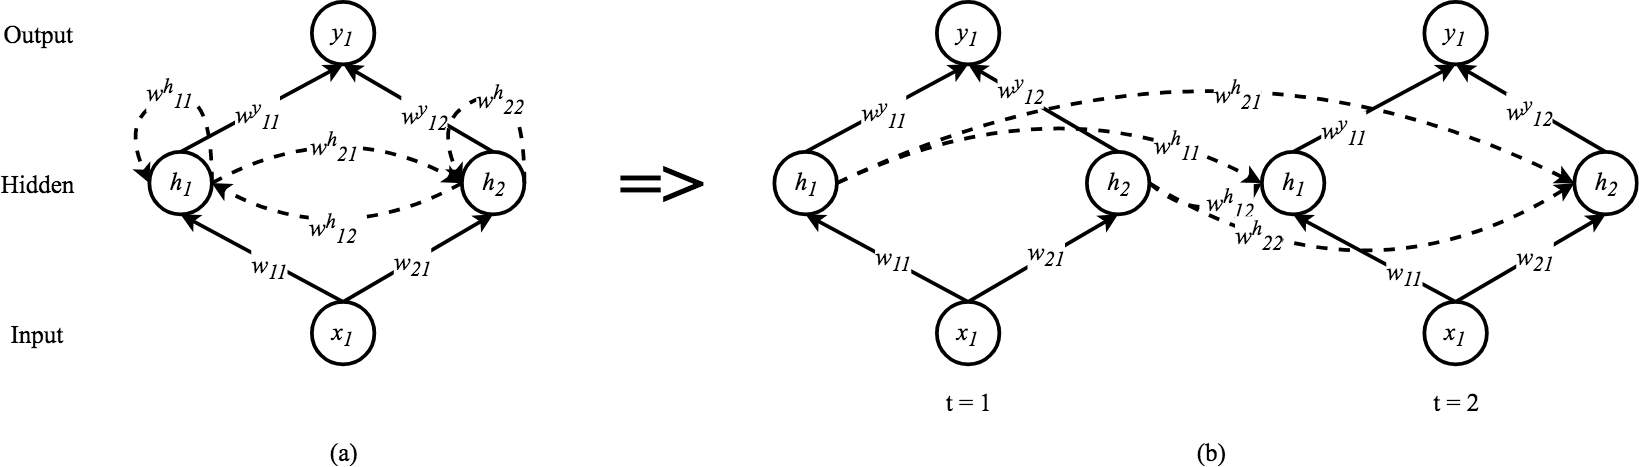
\includegraphics[max width=\textwidth]{recurrent-neural-network}
		\caption{A recurrent neural network with one hidden layer consisting of two units (a). The same neural network in (a) that is unfolded into two time steps (b).}
		\label{fig:recurrent-neural-network}
	\end{figure}
	
	A recurrent neural network is a feed forward neural network with additional connections between the nodes in each hidden layer called recurrent connections. These recurrent connections, connect the weighted output of each hidden node to another hidden node across a single time step. It is important to note that these recurrent connections do not form cycles within a single time step. The weights carried by these recurrent edges represent state that is remembered from one time step to the next and it is through this state that the recurrent neural network learns to infer context\cite{DBLP:journals/corr/Lipton15}.
	
	Figure \ref{fig:recurrent-neural-network} (a) shows a recurrent neural network with one input unit, one output unit and a hidden layer with two units. It also shows the recurrent connections in the hidden layer. Each node in the hidden layer receives inputs from the data point $x$ and from each hidden unit $h$ in the previous time step. Figure \ref{fig:recurrent-neural-network} (b) show the same recurrent neural network that is unfolded into two time steps. Notice that the recurrent connections are no longer depicted as cyclic connections.
	
	Unfolding the recurrent neural network into its component time steps allows us to identify the formula used to calculate the output of each hidden node:
	\begin{equation}
	h_{h}^{(t)} = \sigma(W_{hx} x^{(t)} + W_{hh} h^{(t - 1)} + b_{h})
	\end{equation}
	Where $W_{hx}$ is the weight matrix from the input at the current time step to the hidden unit $h$, $ x^{(t)}$ is input at the current time step, $W_{hh}$ is the weight matrix from the hidden unit $h$ at the previous time step to the same hidden unit at the current time step, $ h^{(t - 1)}$ is the output of the hidden unit $h$ from the previous time step and finally, $b_{h}$ is the bias for the hidden unit $h$\cite{DBLP:journals/corr/Lipton15}.
	
	Unfolding recurrent neural networks also help us visualize them as deep architectures. Each time step can be considered a layer in a deep neural network. This allows us to use the backpropagation algorithm to train recurrent neural networks. A variation of the backpropagation algorithm is used called backpropagation through time (BPTT) \cite{DBLP:journals/corr/Lipton15}.
	
	\subsubsection{Long Short-Term Memory Units}
	
	RNNs encounter difficulties when modeling arbitrary long sequences. When training RNNs on longer sequences the internal weights become too small to be able to capture any context. This is know as the vanishing gradient problem and long short-term memory units (LSTMs) were introduced to overcome this problem\cite{DBLP:journals/corr/Lipton15}. LSTMs employ gating elements that select which parts of the context the unit should "remember" and the parts that it should "forget"\cite{LSTM}.  
	
	\section{Theory}
	
	\subsection{Improving Accuracy using Symbols}
	
	In section \ref{sec:introduction-synopsis} we discussed how learning in individual humans is hampered by the presence of effective local minima, which can be due to an insufficient number of training examples. However, societies develop languages and communication techniques that allow individuals to share knowledge with one another. Through this social interaction, an individual human learner can overcome these difficulties\cite{DBLP:journals/corr/abs-1203-2990}.
	
	Artificial neural networks also experience difficulty in discovering the desired decision function when training with a limited dataset. This is due to the existence of many local minima in the hypothesis space. Just as humans overcome this difficulty with the aid of clear symbols, as represented in interactions with other individuals, we hypothesize that the introduction of clear and consistent symbols of the same concept to an artificial neural network will also help the artificial model overcome the challenge of training with an impoverished dataset.
	
	We believe that learning a concept task from noisy inputs can benefit from learning the same task from clear and consistent symbols of the same concept.  Representation created in the layers for mapping the symbolic inputs to outputs that correctly identify the concept can be used as a scaffold for mapping the noisy inputs to the same outputs. In this way the, weight updates associated with the symbolic inputs guide the back-propagation algorithm to areas of weight space that have fewer suboptimal local minima. The weight updates associated with the noisy inputs will piggy back on the movement along this trajectory because the gradient of the error with respect to the weights will be highest in this direction. This form of inductive bias results in a model that has a higher accuracy than if learned with only the noisy inputs.
	
	\subsection{Approach}
	
	To demonstrate this hypothesis we will construct several neural network models that learn to do basic arithmetic operations on images of handwritten digits(figure \ref{fig:model-input-output}). When properly trained the models can be presented with two images, each representing a single digit, and the network would be able to output a vector, consisting of two one-hot values, representing the result of the operation. One-hot vectors are vectors that have all their features set to 0 except for the feature corresponding to the value being represented. That feature is set to 1. Figure \ref{fig:one-hot-vector} shows an example of a one-hot vector for the number 2.
	
	\begin{figure}
		\centering
		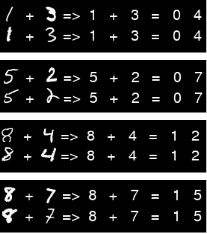
\includegraphics[max width=\textwidth]{model-input-output}
		\caption{Examples of noisy inputs along with clean symbolic inputs and the results of their addition.}
		\label{fig:model-input-output}
	\end{figure}
	
	Alongside the handwritten digit inputs, the models will also have another input channel consisting of a symbolic signal. This channel represents the common language exhibited by human learners. The symbols will be made up of two images containing the same digits clearly rendered in a standard font. Figure \ref{fig:symbols} shows what the clear symbols would look like.
	
	Several types of models will be developed and analyzed. Section \ref{sec:methodology} provides an overview of these models. Some of the models will be trained with the presence of symbols and other will be trained without. All testing will be performed without symbolic information to simulate the behavior of an independent agent. The results will be compared and analyzed to determine the effect of symbols on the effectiveness of the models.
	
	\begin{figure}
		\centering
		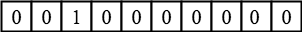
\includegraphics[max width=\textwidth]{one-hot-vector}
		\caption{A one-hot vector representing the number 2.}
		\label{fig:one-hot-vector}
	\end{figure}
	
	\begin{figure}
		\centering
		
\includegraphics[max width=\textwidth]{symbols}
		\caption{Examples of the symbolic data that will be used to train the models.}
		\label{fig:symbols}
	\end{figure}
	
	\subsubsection{Multimodal Learning}
	
	\begin{figure}
		\centering
		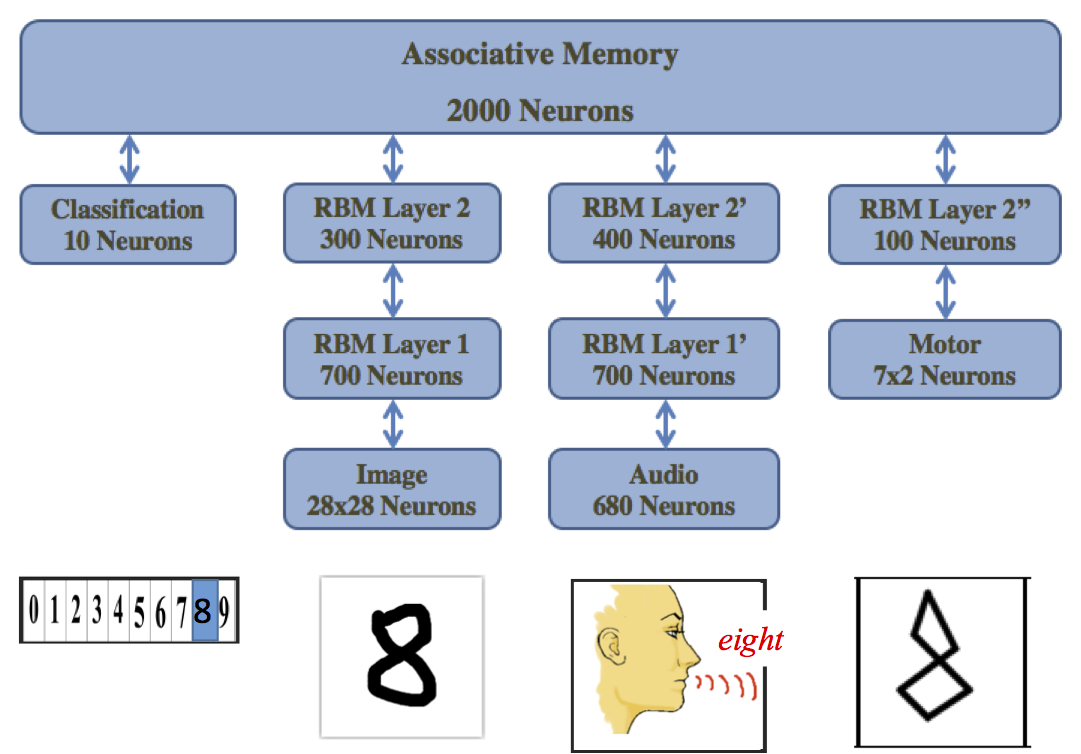
\includegraphics[max width=\textwidth]{multimodal-learning}
		\caption{Multimodal model trained to communicate digits using several mediums.}
		\label{fig:multimodal-learning}
	\end{figure}
	
	Recent work by Igbal and Silver (FLAIRS-2016 Best Paper Award)\cite{iqbal2016scalable} inspired by work by Hinton et al.\cite{Hinton:2006:FLA:1161603.1161605} and Srivastava et al.\cite{JMLR:v15:srivastava14b} has shown that it is possible to develop a multimodal deep learning system for learning a noisy handwritten digit using four sensor/motor channels (visual, audio, robotic, and symbolic) and an associative layer that ties all channels together.  After training, the presentation of a digit (sound, image, drawing) at the visible nodes of the model activates all other channels to create their associated reconstruction at their respective visible nodes. Each channel provides additional information that helps the other channels more accurately reconstruct the output. Figure \ref{fig:multimodal-learning} depicts the architecture that was developed as part of that work.
	
	The symbolic channel outputs the cleanest and clearest signal as to what digit the multimodal deep learning system "thinks" what the given input on the other channel is. The symbolic channel also provides the cleanest and clearest input to assist other channels to generate the correct reconstructions at their visible nodes. This led us to a paper by Yoshua Bengio\cite{DBLP:journals/corr/abs-1203-2990} that discusses the value of symbols (ie. language) in helping individuals to learn concepts (like "cat") better without having to see all possible examples of that concept. This has a profound impact upon the development of our culture and the human species. 
	
	The multimodel system discussed above inspired us to consider developing learning agents that learn to perform arithmetic operations using noisy channels but which can at times also receive concise information on a symbolic channel about the data on the noisy channels.
	
	\subsection{Refinement of Objectives}
	
	To summarize, the objectives of my research are to:
	
	\begin{itemize}
		\item Simulate the process of social interaction amongst human learners using artificial neural networks. A neural network model will represent a single learner. The symbolic channel introduced will represent input provided through interaction with other individuals in the group.
		\item Demonstrate that the existence of such interactions can significantly improve the accuracy of training neural networks.
	\end{itemize}
	
	\section{Methodology} \label{sec:methodology}
	
	\subsection{Dataset Preparation}
	
	\subsubsection{MNIST Dataset}
	
	All experiments that will be conducted will use the MNIST dataset of handwritten digits. This is a database of images of handwritten digits along with labels indicating the values represented. Each digit is normalized and centered in a 28x28 pixel image. The dataset consists of 60,000 training examples and 10,000 test examples. MNIST is very popular among researchers that need to quickly test machine learning techniques since the dataset is already pre-processed \cite{MNIST}.
	
	\subsubsection{Preparation}
	
	The models will be trained to perform addition on single digit inputs from the range of 0 to 9. The dataset is compiled by randomly sampling 10 examples from each combination. For example the 0 + 0 combination has 10 different examples from the MNIST dataset, the 0 + 1 combination has another 10 examples and so on.
	
	The examples under each combination will then be split into 5 sets, 2 examples each. 5-fold cross-validation will be used to train the models were each iteration uses 3 of the 5 sets for training, one set for validation and the remaining set for testing. The mean accuracy and standard deviation will then be calculated and used to compare the experiments graphically and using an hypothesis t-Test to check the statistical difference of the means.
	
	\subsection{Network Architectures and Experiments}
	
	We view modeling arithmetic operations as modeling sequences. An arithmetic expression is expressed as a series of numbers and operators that are processed one at a time. Therefore, our experiments use recurrent neural networks extensively. The experiments performed have two main goals:
	\begin{itemize}
		\item To show that it is possible to create a deep recurrent neural network model that can learn to perform all four basic arithmetic operations (addition, subtraction, multiplication and division) more efficiently and effectively with the presence of symbols than without.
		\item To attempt to build models that can explain their errors by showing that a mathematical miscalculation is the result of miss-classifying a noisy input and that the addition of symbols improves the classification process and therefore improves the accuracy of the calculations
	\end{itemize}
	
	\subsubsection{Sequential Models}
	
	\begin{figure}
		\centering
		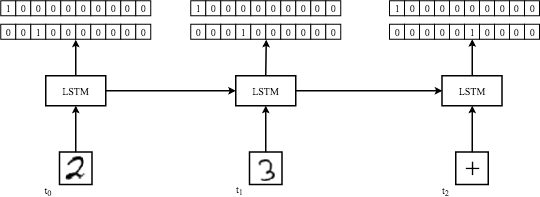
\includegraphics[max width=\textwidth]{sequential-model}
		\caption{A recurrent neural network acting as a sequential adder. The network performs classification on the inputs which can act as symbols to the adder.}
		\label{fig:sequential-model}
	\end{figure}
	
	The first set of models attempt to show that the presence of symbols improves the effectiveness of training neural network models that are trained on limited datasets. This set of models is based on recurrent neural networks, specifically those that use Long Short-Term Memory (LSTM) units. Two methods of providing symbolic information will be examined. The first is based on having a symbolic channel alongside the noisy channel. The other is based on providing classification labels associated with each noisy input during training.
	
	When examining the presence of symbolic data alongside the noisy inputs, we will build recurrent network models that accept 1568 input units. 784 units would be used for one 28x28 handwritten digit and the remaining 784 units will be used for another 28x28 image representing the clear symbol. The operands are fed to the network sequentially (one at a time) and the output is evaluated after the second operand is provided. The networks will be training to perform one operation only to simplify the training set.
	
	When training these models, we will first train with the symbolic channel set to a consistent value (indicating don't care) to simulate a model trained without the presence of symbols. Then we will train another model where the symbols will be provided. When testing the trained models, only noisy data will be provided with the symbolic channel set to the consistent don't care value. The accuracy of both of these attempts will be compared to understand the effect of the presence of symbols on the effectiveness of training.
	
	With the second variation, the network will accept 784 input units representing a 28x28 handwritten digit. The operation operands are fed one at a time. Every time a digit is provided, the model will produce the classification label of that digit on the output vector. If an operator is provided to the network, the model will output the result of the operation of the previous inputs. Figure \ref{fig:sequential-model} shows an example of such a model. Teaching the network to properly classify the inputs before performing the operation is similar to training the model using symbolic input. The LSTM layers should be able to maintain the classes learned within their context, therefore, providing the same utility a symbolic channel would provide.
	
	Similar to how we trained the first variation, we start by using a consistent value for the class labels across all classes of digits. This should behave like a model that was trained without symbols. Then we train another model with proper digit classes provided. The accuracy of both these models will be compared and analyzed to confirm any findings that result from the other class of sequential models. In addition to these models, five other models will be trained one with 0\% classification data, the second with 25\%, the third with 50\%, the forth with 75\% and finally the fifth with 100\% of the classification data provided. The effect on accuracy given the amount of symbolic information provided will then be charted and analyzed.
	
	\subsubsection{Arbitrarily Long Sequences}
	
	So far, we've been only considering arithmetic expressions consisting of only two operands and one arithmetic operator. Our goal is to construct deep neural network models that represent a mathematical system. We would then train that system with and without the presence of symbols to determine the effect of these symbols on the system's accuracy on an independent test set. In order to develop this system, our models must be able to interpret arithmetic expressions that consist of an arbitrary number of operations as well as having sequences that include more than one operator type. The sequential model discussed above will therefore be modified to output four vectors instead of two to allow for larger outputs. Similar to the previous experiments, several models will be constructed with varying amounts of symbolic information.
	
	\subsubsection{Understanding the Behavior of Models Trained with Symbols}
	
	To accomplish our second goal of building models that explain the reasons for their errors, we will construct and train an LSTM based recurrent neural network that accepts 784 input units. Like the previous models, these represent the 28x28 pixels of a handwritten digit or an operator. Unlike the previous models, this one will have 5 one-hot vectors as output. The first will project what the network "understands" to be the first operand after every step of the sequence. The second will represent the second operand. The third vector will show the operator and finally the remaining two will show the results of the operation.
	
	During training, all this information will be included in the training set. When testing however, the values of each vector will be analyzed to understand the patterns shown if any. For examples, if the sequence of 5 + 5 is presented as an input, but the result was calculated as 5 instead of 10, we might notice that during the final input, the network shows us that it understands the first operand to be a 0, that would justify why the output was 5 (0 + 5 is 5).
	
	Other techniques to capture the models "understanding" of the inputs will also be investigate. Specifically analyzing the visual representation of the operands compared to the resulting classes and results of the operation. This qualitative technique involves rendering the input sequences along with their intermediate and final outputs to understand which combinations the model recognizes correctly from those that it does not. The aim here is to understand the results when we consider factors like elements of the handwritten digits resembling other digits or digits that were misclassified but provided correct results based on the classes identified as opposed to the actual handwritten inputs. Understanding factors like these could provide some insight into how the network behaves internally. For example, if the network is learning to represent an algorithm or if it's simply learning to perform pattern matching.
	
	Finally, we will modify the way we generate these training sets so that not all combinations of operands are provided to the networks during training. The models must still be provided all the numbers in one form since otherwise the network won't be able to use numbers that it has never seen before. The goal of this partial training technique is to see how well the model performs on combinations of operands it has never seen before. If the performance is reasonable, this would indicate that the model is indeed learning the underlying algorithm behind the operations as opposed to simply memorizing the combinations it sees.
	
	\subsection{Technical Specifications}
	
	The following tools will be used to construct and test the models:
	
	\begin{itemize}
		\item Python 2.7.x
		\item TensorFlow
		\item Keras
		\item NumPy
		\item Matplotlib
		\item Python Image Library (PIL)
	\end{itemize}
	
	Access to a Linux server with Nvidia CUDA support will be required to speed up model training and testing.
	
	\section{Thesis Outline}
	
	The following is a list of the major sections and subsections of the thesis document:
	
	\begin{itemize}
		\item Chapter 1: Introduction
		\begin{itemize}
			\item Introduction to Machine Learning
			\begin{itemize}
				\item Neural Networks
				\item Challenges in Training Neural Networks
			\end{itemize}
			\item Learning with Symbols
			\item Research Objective and Scope
			\item Thesis Outline
		\end{itemize}
		\item Chapter 2: Background
		\begin{itemize}
			\item Artificial Neural Networks
			\begin{itemize}
				\item The Perceptron
				\begin{itemize}
					\item Gradient Descent Algorithm
					\item Activation Functions
					\item Adam Optimizer
				\end{itemize}
				\item Feed Forward Neural Networks
				\begin{itemize}
					\item Backpropagation Algorithm
					\item Stochastic Approximation and Batch SGD
					\item The Problem of Overfitting 
				\end{itemize}
				\item Deep Learning
				\begin{itemize}
					\item The Depth-Breadth Tradeoff
					\item Parallelizing Training
				\end{itemize}
			\end{itemize}
			\item The Problem of Local Minima
			\item Sequence Modeling
			\begin{itemize}
				\item Recurrent Neural Networks
				\begin{itemize}
					\item Backpropagation Through Time
				\end{itemize}
				\item Vanishing Gradient Problem
				\item Long Short-Term Memory Units
			\end{itemize}
		\end{itemize}
		\item Chapter 3: Theory
		\begin{itemize}
			\item Hypothesis
			\begin{itemize}
				\item Multi-Task Learning
			\end{itemize}
			\item Approach
			\begin{itemize}
				\item The MNIST Dataset
				\item Multimodal Learning
				\item Sequential Models
				\item Multi-Operator Models
				\item Arbitrarily Long Sequences
			\end{itemize}
			\item Understanding the Behavior of Symbols
			\begin{itemize}
				\item Qualitative Analysis
				\item Partial Training
			\end{itemize}
		\end{itemize}
		\item Chapter 4: Empirical Studies
		\begin{itemize}
			\item Data Preparation
			\item Environment
			\item Experiment: Sequential Models
			\begin{itemize}
				\item Objective
				\item Method
				\item Results
				\item Discussion
			\end{itemize}
			\item Experiment: Arbitrarily Long Sequences
			\begin{itemize}
				\item Objective
				\item Method
				\item Results
				\item Discussion
			\end{itemize}
			\item Experiment: Multi-Output Model
			\begin{itemize}
				\item Objective
				\item Method
				\item Results
				\item Discussion
			\end{itemize}
			\item Experiment: Partial Training
			\begin{itemize}
				\item Objective
				\item Method
				\item Results
				\item Discussion
			\end{itemize}
			\item Discussion
		\end{itemize}
		\item Chapter 5: Conclusion and Future Work
		\begin{itemize}
			\item Findings and Outcomes
			\item Conclusion
			\item Future Work
		\end{itemize}
	\end{itemize}
	
	\section{Progress Timeline}
	
	The following is a breakdown of the proposed timeline to submit the final version of the thesis:
	
	\begin{itemize}
		\item June 2018
		\begin{itemize}
			\item Completed Parallel Model experiments
		\end{itemize}
		\item July 2018
		\begin{itemize}
			\item Worked on Sequential Model experiments
			\item Completed Chapter 1: Introduction
		\end{itemize}
		\item August 2018
		\begin{itemize}
			\item Completed Sequential Model experiments
			\item Completed Chapter 3: Theory
			\item Completed Chapter 2: Background
		\end{itemize}
		\item September 2018
			\begin{itemize}
				\item Finalize experiments
				\item Complete Chapter 4: Empirical Studies
			\end{itemize}
		\item October 2018
			\begin{itemize}
				\item Complete Chapter 5: Conclusion and Future Work
			\end{itemize}
		\item November 2018
			\begin{itemize}
				\item Finalize Thesis
				\item Submit Thesis Draft
			\end{itemize}
		\item December 2018
		\begin{itemize}
			\item Thesis Defence
			\item Thesis Corrections
			\item Submit Final Version
		\end{itemize}
	\end{itemize}
	
	\bibliographystyle{unsrt}
	\bibliography{proposal}
	
\end{document}